\section{Comment résoudre le problème}
\subsection{Définir le problème}
\paragraph{}
Le problème que nous essayons de résoudre est de suivre précisément les yeux pour pouvoir déplacer le curseur de la souris.
Cela fait partie d'une gamme plus large de problèmes de \emph{Computer Vision}, et plus précisément de \emph{eye tracking}.
Selon \cite{eye_tracking}, le suivi des yeux est ``le processus de mesure du point de vue (où l'on regarde) ou du mouvement d'un œil par rapport à la tête''.
% The problem we're trying to solve is accurately tracking one's eyes in order to move the mouse cursor.
% This is part of a broader range of \emph{Computer Vision} problems, and more precisely \emph{eye tracking}.
% According to \cite{eye_tracking}, eye tracking is ``the process of measuring either the point of gaze (where one is looking) or the motion of an eye relative to the head''.
\paragraph{}
Sachant cela, nous allons nous attaquer à ce problème en utilisant \emph{l'Intelligence Artificielle}, car c'est devenu aujourd'hui un moyen viable de résoudre ces problèmes.
Nous allons donc traiter un problème \emph{d'Apprentissage Automatique}, plus précisément un problème \emph{d'Apprentissage profond}.
% Knowing these, we will tackle this problem using \emph{Artificial Intelligence}, since this has nowadays become a viable way of solving such problems.
% We will therefore be dealing with a \emph{Machine Learning} problem, more precisely a \emph{Deep Learning} one.
\paragraph{}
Les tâches d'Apprentissage Profond peuvent être supervisées, semi-supervisées ou non supervisées.
Nous nous concentrerons sur les tâches \emph{supervisées} et nous traiterons notre problème comme l'une d'entre elles.
Cela signifie que nous allons d'abord acquérir quelques données d'apprentissage, qui consisteront en des images de webcam marquées par la position du curseur de la souris.
De cette façon, notre algorithme apprendra où le curseur de la souris doit se trouver, en fonction de l'endroit où l'utilisateur regardait lorsque l'image a été prise.
% The Deep Learning tasks can be either supervised, semi-supervised or unsupervised.
% We'll focus on the \emph{supervised} tasks and we'll treat our problem as one of those.
% That means that we will first acquire some \emph{learning data}, which will consist in webcam images labeled with the position of the mouse cursor.
% That way, our algorithm will learn where the mouse cursor should be, depending on where the user was looking when the image was taken.

\subsection{Le neurone artificiel}
\paragraph{}
Avant d'entrer dans des architectures d'Apprentissage Profond plus sophistiquées, nous devons d'abord examiner le neurone artificiel.
En bref, il s'agit d'un modèle formel et simplifié de neurone biologique.
Il peut nous aider à faire la \emph{classification binaire} à l'aide de la formule suivante:
% Before going into more sofisticated deep learning architectures, we first have to take a look at the artificial neuron.
% Put shortly, it is a formal, simplified model of a biological neuron.
% It can help us do \emph{binary classification} using the following formula:
$$
y = \varphi (w * x + b)
$$
% \begin{equation}
%     f(x) =
%     \begin{cases}
%       1, & \text{if}\ w * x + b > 0 \\
%       0, & \text{autrement}
%     \end{cases}
% \end{equation}

\paragraph{}
Dans la formule ci-dessus, $x$ est un vecteur de valeurs réelles, représentant notre entrée, $w$ est un vecteur de valeurs réelles, appelé \emph{poids} et $b$ est le \emph{biais}.
Le produit $w * x$ représente le produit scalaire et est égal à $w * x = \sum _{i=1}^{n}w_{i}x_{i}$, $n$ étant la longueur de notre entrée.
% In the formula above, $x$ is a vector of real values, representing our input, $w$ is a vector of real values, called \emph{weights} and $b$ is the \emph{bias}.
% The product $w * x$ represents the scalar product and is equal to $w * x = \sum _{i=1}^{n}w_{i}x_{i}$, with $n$ being the length of our input.

\paragraph{}
Le résultat de la classification est donné par $\varphi$, qui est appelé une \emph{fonction d'activation}.
Si cette fonction sert de seuil, elle effectuera une classification binaire, donnant soit $0$ soit $1$.
Nous pourrions même utiliser une fonction d'activation telle que $\varphi(x) = x$ qui ne nous donnera pas une classification binaire, mais pourrait nous aider à résoudre des problèmes de régression linéaire.
% The result of the classification is given by $\varphi$, which is called an \emph{activation function}.
% If that acts as a threshold, then it will make binary classification, giving either $0$ or $1$.
% We could even use an activation function such as $\varphi(x) = x$ which will not give us a binary classification, but could help us solve linear regression problems.

\begin{figure}[H]
    \centering
    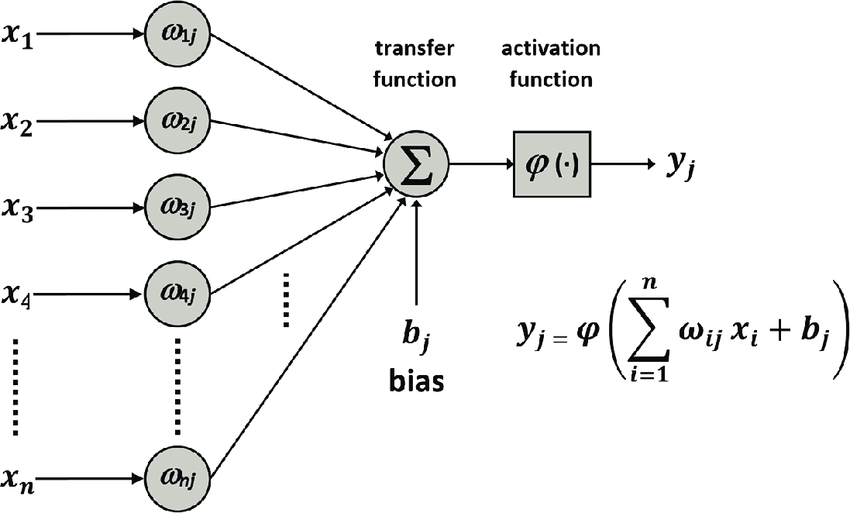
\includegraphics[width=\textwidth]{artificial_neuron.png}
    \caption{Schéma d'un neurone artificiel\\Source: \href{https://www.researchgate.net/figure/Scheme-of-a-perceptron-A-nonlinear-activation-function-BULLET-is-applied-to-the_fig3_315788933}{ResearchGate}}
\end{figure}


\subsection{Les réseaux de neurones}
\paragraph{}
Le ``cheval de bataille'' des problèmes de vision par ordinateur est le réseau de neurones artificiels.
Celui-ci est, comme son nom l'indique, composé de plusieurs neurones artificiels, répartis sur plusieurs couches.
% The main ``workhorse'' for Computer Vision problems is the Artificial Neural Network.
% This is, as the name suggest, composed of multiple artificial neurons, distributed over multiple layers.

\begin{figure}[H]
    \centering
    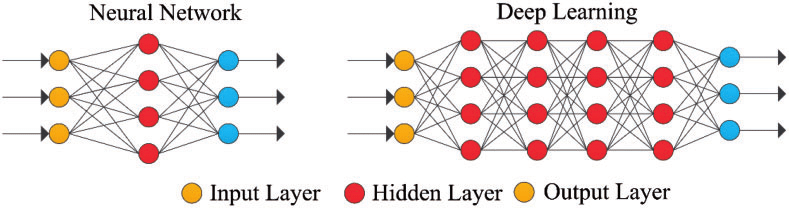
\includegraphics[width=\textwidth]{ann.png}
    \caption{Schéma d'un neurone artificiel\\Source: \href{https://www.researchgate.net/figure/Deep-learning-diagram_fig5_323784695}{ResearchGate}}
\end{figure}

% ========== Strategy Section ==========
\section{Strategie}

\subsection{Obtenir des données}
\paragraph{}
Il est bien connu qu'un algorithme d'Apprentissage Automatique n'est bon que si les données que nous lui fournissons le sont aussi.
C'est incroyablement important, c'est pourquoi je vais m'efforcer de rassembler autant de données que possible, ainsi que d'autres informations que je pourrais trouver importantes.
% It is widely known that a Machine Learning algorithm is only as good as the data we feed it.
% This is incredibly important, so I will focus on gathering as much \emph{raw data} as possible, along with other information I might find important.

\paragraph{}
Un autre point essentiel est \emph{traitement des données} et \emph{analyse des données}.
Le premier concerne le nettoyage de l'ensemble des données des instances inutiles et la mise en forme des données recueillies dans un format utilisable pour nos réseaux neuronaux.
Nous examinerons également comment nous pouvons obtenir des informations supplémentaires qui pourraient être utiles à partir de nos images.
% Another essential point is \emph{data processing} and \emph{data analysis}.
% The first one is concerned about cleansing the dataset of useless instances and bringing the data we gathered into a usable format for our neural networks.
% We will also look into how we can derive additional information that could be useful based on our images.

\subsection{Perceptrons multicouches}
\paragraph{}
Un type particulier de réseaux neuronaux est le réseau multicouche Perceptron.
Ce sera ma première expérience et le point de départ pour tenter de résoudre le problème.
% A special kind of neural networks is the Multilayer Perceptron Network.
% This will be my first experiment and the starting point for trying to solve the problem.

\paragraph{}
En utilisant ceci, je vais essayer de résoudre le premier objectif \ref{chapter-introduction-first-objective}, et c'est approximativement de prédire où l'utilisateur regarde.
Je vais d'abord essayer avec une grille plus petite de 2x2, puis je passerai à une grille de 3x3.
% Using this, I'll try to solve the first objective \ref{chapter-introduction-first-objective}, and that is approximately predicting where the user is looking.
% I'll try first with a smaller 2x2 grid, then move up to a 3x3 grid.

\subsection{Réseau neurones convolutifs}
\paragraph{}
Une étape supplémentaire consistera à utiliser les réseaux neuronaux convolutifs, une architecture de pointe pour travailler avec des images.
Cela pourrait permettre d'atteindre un objectif plus préférable, à savoir prévoir exactement l'emplacement du curseur de la souris en fonction de l'endroit où l'utilisateur regarde.
% A step further will be to use Convolutional Neural Networks, a state of the art architecture for working with images.
% This could help to reach a more preferable objective, and that is predicting exactly where the mouse cursor would be based on where the user is looking.

\subsection{Recherche d'autres méthodes}
\paragraph{}
Après avoir expérimenté les méthodes ci-dessus, je vais rechercher de meilleures façons de résoudre ce problème.
Cela pourrait signifier un meilleur traitement des données, un meilleur réglage des réseaux de neurones, etc.
% After experimenting with the methods above, I will research on better ways of solving this problem.
% That could mean better data processing, better tuning of the neural networks and so on.
% ~~~~~~~~~~ Strategy Section ~~~~~~~~~~